\documentclass{report}


%% IF YOU HAVE FONTS INSTALLED
%\usepackage{mtpro2}
%\usepackage{mathtime}
\usepackage[style=trad-plain,backref=true,url=false,isbn=false,alldates=year,sortcites=true,maxnames=9]{biblatex}
\addbibresource{dg-special.bib}
\addbibresource{dg.bib}
\renewbibmacro{in:}{%
  \ifentrytype{article}{}{\printtext{\bibstring{in}\intitlepunct}}}
\usepackage{geometry}
\usepackage{amssymb}
\usepackage{latexsym, amsmath, amscd,amsthm}
\usepackage{thmtools}
\usepackage{newtxtext,newtxmath}
\usepackage{mathtools}
\usepackage{graphicx}
\usepackage[percent]{overpic}
%\usepackage{pdfsync}
\usepackage{units}
\usepackage{tikz}
\usepackage{diagbox}
\usepackage{xcolor}
\definecolor{linkblue}{HTML}{003d73}
\definecolor{linkgreen}{HTML}{006161}
\definecolor{linkred}{HTML}{a11950}
\usepackage{hyperref}
\hypersetup{ 
	pdftitle={Introduction to Differential Manifolds},
	pdfauthor={Clayton Shonkwiler},
	pdfsubject={differential geometry},
	pdfkeywords={manifolds, vector fields, differential forms, Lie groups, homogeneous spaces, Riemannian geometry},
	colorlinks=true,
	linkcolor=linkblue,
	citecolor=linkgreen,
	urlcolor=linkred
}
\PassOptionsToPackage{caption=false,labelformat=empty}{subfig}
\usepackage[lofdepth]{subfig}
\usepackage[export]{adjustbox}
\usepackage{algorithm}
\usepackage{algorithmicx}
\usepackage{algpseudocode}
\usepackage{booktabs}
\usepackage{authblk}
\usepackage{enumitem}

\usepackage{supertabular,multicol,ifthen,multirow}

\usepackage{array}
\newcolumntype{L}[1]{>{\raggedright\let\newline\\\arraybackslash\hspace{0pt}}m{#1}}
\newcolumntype{C}[1]{>{\centering\let\newline\\\arraybackslash\hspace{0pt}}m{#1}}
\newcolumntype{R}[1]{>{\raggedleft\let\newline\\\arraybackslash\hspace{0pt}}m{#1}}

% \usepackage{cite}
\usepackage[nameinlink,capitalize]{cleveref}

\makeatletter
\let\mcnewpage=\newpage
\newcommand{\TrickSupertabularIntoMulticols}{%
\renewcommand\newpage{%
    \if@firstcolumn%
        \hrule width\linewidth height0pt%
            \columnbreak%
        \else%
          \mcnewpage%
        \fi%
}%
}
\makeatother

\graphicspath{{./figs/}}

%\usepackage{clrscode}

% \def\figdir{figs/}
% \graphicspath{\figdir}

\crefname{figure}{Figure}{Figures}



\newtheorem{theorem}{Theorem}[section]
\newtheorem{lemma}[theorem]{Lemma}
\newtheorem{proposition}[theorem]{Proposition}
\newtheorem{corollary}[theorem]{Corollary}
\newtheorem*{mainthm}{Theorem~\ref*{thm:main}}

\theoremstyle{definition}
\newtheorem{definition}[theorem]{Definition}
\newtheorem{example}[theorem]{Example}
\newtheorem{conjecture}[theorem]{Conjecture}
\newtheorem{remark}[theorem]{Remark}
\newtheorem*{notation}{Notation}


\newcommand{\R}{\mathbb{R}}
\newcommand{\I}{\mathbf{i}}
\newcommand{\Z}{\mathbb{Z}}
\newcommand{\from}{\co\!\!}
\def\co{\colon\thinspace}


\renewcommand{\theenumi}{(\roman{enumi})}
\renewcommand{\labelenumi}{(\roman{enumi})}

\newcommand{\seqnum}[1]{\href{http://oeis.org/#1}{#1}}
\newcommand{\ent}[3]{E_{#1,#2}^{(#3)}}

\let\oldReturn\Return
\renewcommand{\Return}{\State\oldReturn}


%% BibLaTeX junk
%-----------------

% Change backref style
\DefineBibliographyStrings{english}{%
  backrefpage = {$\uparrow$},% originally "cited on page"
  backrefpages = {$\uparrow$},% originally "cited on pages"
  page = {p\adddot},
  pages = {pp\adddot},
}

% Drop fields from output
\DeclareSourcemap{
  \maps{
    \map{
      \step[fieldset=pagetotal, null]
	  \step[fieldset=pubstate, null]
    }
  }
}

% New eprint types
\DeclareFieldFormat{eprint:urn}{%
  \mkbibacro{URN}\addcolon\space
  \ifhyperref
    {\href{https://nbn-resolving.org/urn:#1}{\nolinkurl{#1}}}
    {\nolinkurl{#1}}}
\DeclareFieldAlias{eprint:URN}{eprint:urn}
\DeclareFieldFormat{eprint:hal}{%
  \mkbibacro{HAL}\addcolon\space
  \ifhyperref
    {\href{https://hal.science/#1}{\nolinkurl{#1}}}
    {\nolinkurl{#1}}}
\DeclareFieldAlias{eprint:HAL}{eprint:hal}
\DeclareFieldFormat{eprint:numdam}{%
  Numdam\addcolon\space
  \ifhyperref
    {\href{http://www.numdam.org/item/#1}{\nolinkurl{#1}}}
    {\nolinkurl{#1}}}
\DeclareFieldAlias{eprint:Numdam}{eprint:numdam}
\DeclareFieldFormat{eprint:ark}{%
  \mkbibacro{ARK}\addcolon\space
  \ifhyperref
    {\href{https://n2t.net/ark:#1}{\nolinkurl{#1}}}
    {\nolinkurl{#1}}}
\DeclareFieldAlias{eprint:ARK}{eprint:ark}
\DeclareFieldFormat{eprint:zbl}{%
  Zbl\addcolon\space
  \ifhyperref
    {\href{https://zbmath.org/#1}{\nolinkurl{#1}}}
    {\nolinkurl{#1}}}
\DeclareFieldAlias{eprint:Zbl}{eprint:zbl}
\DeclareFieldFormat{eprint:mr}{%
  \mkbibacro{MR}\addcolon\space
  \ifhyperref
    {\href{https://mathscinet.ams.org/mathscinet-getitem?mr=#1}{\nolinkurl{#1}}}
    {\nolinkurl{#1}}}
\DeclareFieldAlias{eprint:MR}{eprint:mr}

%-----------------



\hyphenation{pa-ram-e-tri-za-tion}

\tikzset{my node/.style = {shape=circle, fill=black, inner sep = 1.5pt, outer sep = 0pt}}


\setlength{\parskip}{3pt}


\newenvironment{coordinates}[1]{
	\nobreak\vfil\penalty0\vfilneg\vtop\bgroup
	\begin{center} \begin{normalsize} #1 \end{normalsize} \end{center} 

		\ttfamily \begin{tiny}\begin{center}
	}{
		\end{center}\end{tiny}\par
		\xdef\tpd{\the\prevdepth}\egroup\prevdepth=\tpd
	}

\title{Introduction to Differential Manifolds}
\author{Clayton Shonkwiler}
\affil{Department of Mathematics, Colorado State University, Fort Collins, CO, USA}

\date{}

\renewcommand\Affilfont{\itshape\small}

\setcounter{MaxMatrixCols}{20}

\begin{document}



\maketitle

\chapter{Manifolds and Vector Fields}

% !TEX root = ../dg.tex

\section{Manifolds and Maps}

The title of this course is ``Introduction to Differential Manifolds,'' which suggests that these \emph{differential manifolds} (or sometimes \emph{differentiable manifolds}), whatever they are, will probably be important. So what is a differential manifold? The name should suggest the answer: they are spaces in which we know what differentiation is supposed to mean. I actually prefer the term \emph{smooth manifold}, so that is what I will use going forward, though this will often just get shortened to \emph{manifold}.

In practice, the idea is to leverage the fact that we already (hopefully!) know how to do calculus in $\R^n$ (this is exactly what MATH 261 is all about), and to translate those techniques to more general spaces. The key insight here is that differentiation is a local operation: to compute a derivative at a point (whether it's a gradient, curl, divergence, directional derivative, whatever), you really only need to know what's going on in a tiny open neighborhood of that point. 

So to get a space on which we can compute derivatives, it's enough to have a space which is ``locally Euclidean'' or ``locally like $\R^n$,'' and this is what manifolds are. Roughly speaking, this means that around any point in a manifold you can find a small open set which looks just like an open set in some $\R^n$, and then we can do calculus on the manifold by translating in a neighborhood of a point to the corresponding set in $\R^n$, where we know what to do.

This is all to say that the point of defining manifolds in the way we are about to (which is extremely non-obvious and unintuitive!) is that these are precisely the spaces in which a suitable generalization of multivariable calculus makes sense.

So what does ``locally like $\R^n$'' actually mean? Here's a standard definition:

\begin{definition}\label{def:manifold}
	A \emph{smooth manifold of dimension $n$} is a Hausdorff, second-countable topological space $M$ together with a family of injective maps $\phi_\alpha\from U_\alpha \to M$ from open sets $U_\alpha \subseteq \R^n$ so that:
	\begin{enumerate}
		\item \label{it:manifold def cover}$\bigcup_\alpha \phi_\alpha(U_\alpha) = M$ (that is, the images of the maps $\phi_\alpha$ cover all of $M$);
		\item \label{it:manifold def overlap}For any $\alpha, \beta$ so that $\phi_\alpha(U_\alpha) \cap \phi_\beta(U_\beta) = W \neq \emptyset$, the sets $\phi_\alpha^{-1}(W)$ and $\phi_\beta^{-1}(W)$ are open sets in $\R^n$ and the maps $\phi_\beta^{-1} \circ \phi_\alpha$ and $\phi_\alpha^{-1} \circ \phi_\beta$ (when restricted to these open sets) are smooth.
		\item \label{it:manifold def maximal}The family $\{(U_\alpha, \phi_\alpha)\}$ is maximal with respect to \ref{it:manifold def cover} and \ref{it:manifold def overlap}.
	\end{enumerate}
	The pairs $(U_\alpha, \phi_\alpha)$ are called \emph{coordinate charts} and the (maximal) collection $\{(U_\alpha, \phi_\alpha)\}$ is called an \emph{atlas}.	
\end{definition}

See \cref{fig:chart} for a visualization of \ref{it:manifold def overlap}, showing the map $\phi_\beta^{-1} \circ \phi_\alpha$ from $\phi_\alpha^{-1}(W) \subseteq \R^n$ to $\phi_\beta^{-1}(W) \subseteq \R^n$.

\begin{figure}[htbp]
	\centering
		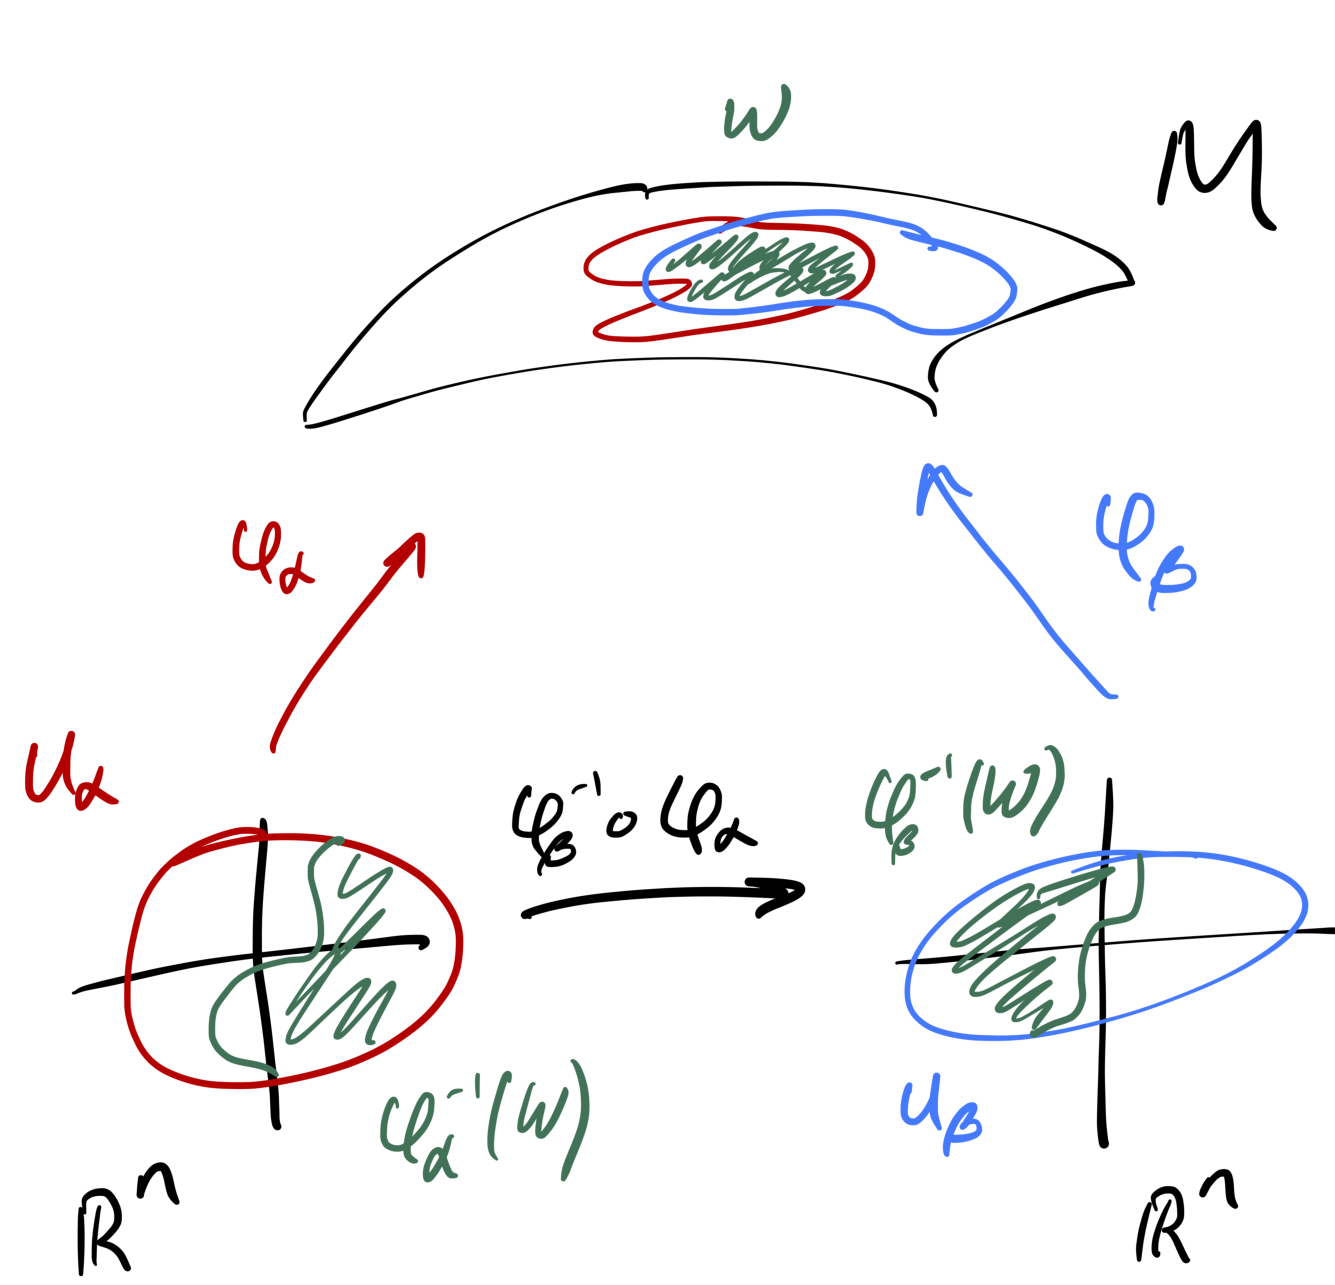
\includegraphics[height=3in]{chart}
	\caption{Transition maps.}
	\label{fig:chart}
\end{figure}

\begin{remark}
	In \ref{it:manifold def overlap} above, ``smooth'' means ``infinitely differentiable'' or, in shorthand, $C^\infty$. What I'm calling \emph{smooth manifolds} are sometimes also called $C^\infty$ \emph{manifolds}. More generally we can talk about $C^\alpha$ manifolds for any integer $\alpha \geq 0$, where we just modify \ref{it:manifold def overlap} to require the maps $\phi_\beta^{-1} \circ \phi_\alpha$ and $\phi_\alpha^{-1} \circ \phi_\beta$ to be $C^\alpha$.\footnote{Recall that a continuous map is $C^\alpha$ if it has $\alpha$ continuous derivatives.} In the special case $\alpha = 0$, this is just a requirement that these maps be continuous, and $C^0$ manifolds are often called \emph{topological manifolds}.
\end{remark}

\begin{example}
	The maximal family containing $(\R^n, \operatorname{id})$ makes $\R^n$ into a smooth manifold.
\end{example}

Of course, most interesting manifolds are not $\R^n$, but the idea of \ref{it:manifold def cover} from \cref{def:manifold} is that you can cover any manifold by a bunch of little open sets (namely, the $\phi_\alpha(U_\alpha)$) that are essentially identical to open sets in $\R^n$ (namely, the $U_\alpha$),\footnote{In topological terms, $U_\alpha$ and $\phi_\alpha(U_\alpha)$ are homeomorphic.} so you can essentially do any local calculation in $\R^n$. It's also very important that the $n$ is always the same here: if $m \neq n$, we're not allowed to have some points with neighborhoods that look like $\R^m$ and some other points whose neighborhoods look like $\R^n$.

If the idea is to use the coordinate charts to transport calculations from the manifold to $\R^n$, then a thing you should be very worried about is that, if a point lies in two different charts, then there are two different ways to do this and they might not be compatible. This is the point of \ref{it:manifold def overlap}: whether you do your calculations in $U_\alpha$ or $U_\beta$, the two are related by a smooth map, so you can easily translate between the two calculations using the change-of-variables formula. Indeed, the usual English-language gloss of \ref{it:manifold def overlap} is that ``transition functions are smooth.''

Finally, \ref{it:manifold def maximal} is a technical condition that in practice is not important. The point of it is simply to ensure uniqueness: if you had a collection of coordinate charts satisfying \ref{it:manifold def cover} and \ref{it:manifold def overlap}, and I took your collection and added some new charts while still satisfying \ref{it:manifold def overlap}, it would be kind of silly to say that you and I were talking about different manifolds. Taking maximal families gives uniqueness since your collection of charts and my collection of charts live in the same maximal family.

% Add discussion that a smooth structure is basically a decision of what should be $C^\infty(M)$, and that, if you don't include \ref{it:manifold def maximal}, then you get ``different'' smooth structures with the same collection of smooth functions.

However, it is certainly possible to have distinct maximal collections on the same space (if there is one that is in some sense standard, then any others are sometimes called ``exotic smooth structures''). At least two Fields Medals have been awarded primarily for finding examples of exotic smooth structures: to John Milnor in 1962 (for finding exotic 7-spheres~\cite{milnorManifoldsHomeomorphic7sphere1956}; it turns out there are exactly 28 distinct smooth structures on $S^7$~\cite{kervaireGroupsHomotopySpheres1963a}) and to Simon Donaldson in 1986 (for finding exotic $\R^4$s~\cite{freedmanTopologyFourdimensionalManifolds1982,donaldsonApplicationGaugeTheory1983,gompfThreeExotic$mathbfR^4$s1983}; it turns out there are uncountably many distinct smooth structures on $\R^4$~\cite{taubesGaugeTheoryAsymptotically1987}). It remains an open problem called the \emph{smooth 4-dimensional Poincaré conjecture} whether there are non-standard differentiable structures on $S^4$.

\begin{remark}
	We often mimic the $\R^n$ notation and indicate the dimension of a manifold $M$ with a superscript; i.e., $M^n$ means that $M$ is an $n$-dimensional manifold, not that we are taking the Cartesian product $M \times M \times \dots \times M$.
\end{remark}

\begin{example}
	$S^n$ the unit sphere in $\R^{n+1}$ is a manifold. Specifically, I claim that the maximal family containing $\{(R^n, \phi_N), (R^n, \phi_S)\}$ makes $S^n$ into an $n$-dimensional manifold, where $\phi_N$ and $\phi_S$ are inverse stereographic projection from the north and south poles, respectively. 
	
	Specifically, with $\vec{x} = (x_1, \dots , x_n) \in \R^n$, define
	\[
		\phi_N(\vec{x}) := \frac{1}{1+\|\vec{x}\|^2}\left(2x_1, \dots , 2x_n, -1+\|\vec{x}\|^2\right)
	\]
	and
	\[
		\phi_S(\vec{x}) := \frac{1}{1+\|\vec{x}\|^2}\left(2x_1, \dots , 2x_n, 1-\|\vec{x}\|^2\right).
	\]
	
	Then $\phi_N$ is the map that sends $\vec{x} \in \R^n$ to the point on the sphere which lies on the line segment connecting $(x_1,\dots , x_n, 0) \in \R^{n+1}$ to the north pole $(0, \dots , 0, 1) \in S^n \subset \R^{n+1}$; see \cref{fig:stereo}. 
	
	\begin{figure}[htbp]
		\centering
			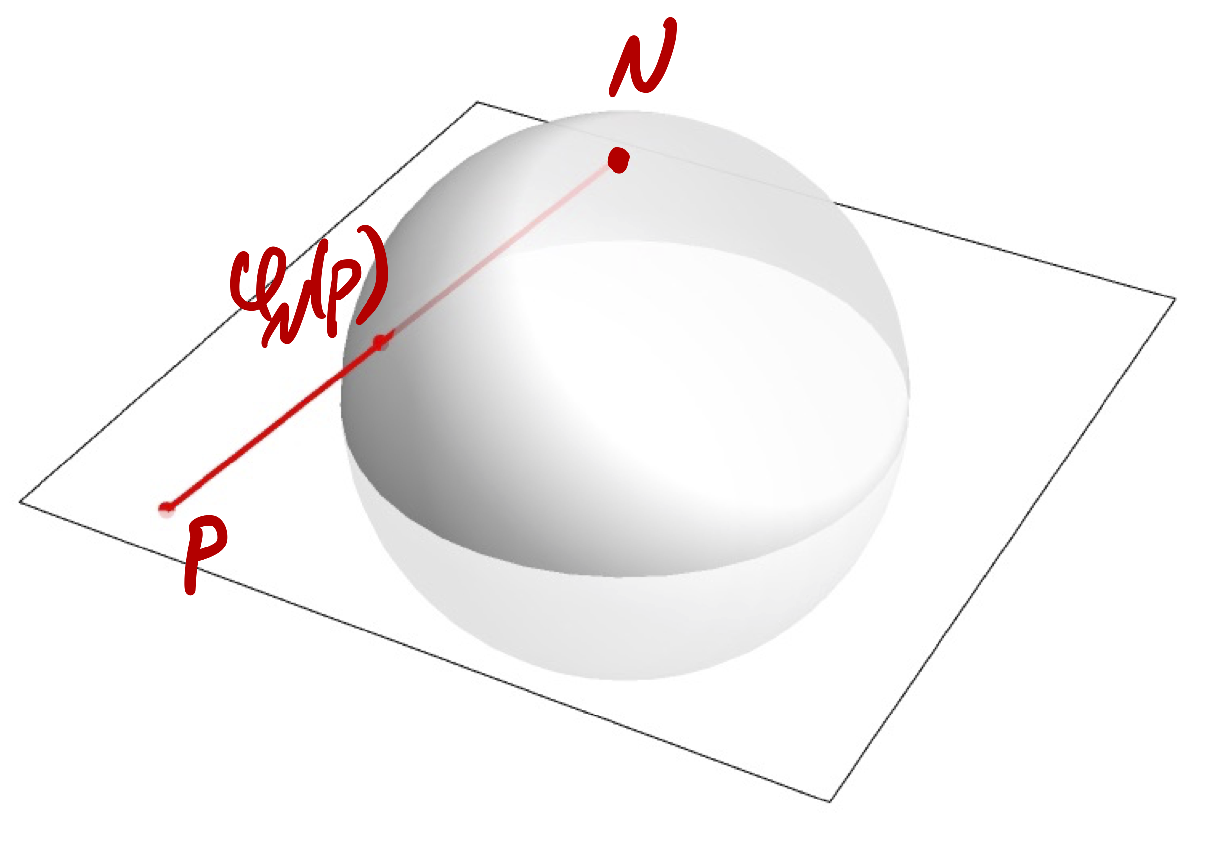
\includegraphics[height=2in]{stereo}
		\caption{Inverse stereographic projection.}
		\label{fig:stereo}
	\end{figure}

To prove the claim, we need to show that \ref{it:manifold def cover} and \ref{it:manifold def overlap} from \cref{def:manifold} are satisfied (\ref{it:manifold def maximal} is automatically satisfied, since we're taking the maximal family containing $\{(\R^n, \phi_N), (\R^n, \phi_S)\}$). 

If we let $N = (0,\dots , 0, 1)$ be the north pole and $S = (0,\dots , 0, -1)$ the south pole, then $\phi_N(\R^n) = S^n \backslash\{N\}$ and $\phi_S(\R^n) = S^n \backslash\{S\}$ and the union is all of $S^n$, so \ref{it:manifold def cover} is satisfied.

For \ref{it:manifold def overlap}, observe that
\[
	W = \phi_N(\R^n) \cap \phi_S(\R^n) = S^n \backslash\{N,S\},
\]
so 
\[
	\phi_N^{-1}(W) = \R^n \backslash\{0\},
\]
which is certainly open, and likewise for $\phi_S^{-1}(W) = \R^n \backslash\{0\}$. So we need to verify that $\phi_N^{-1} \circ \phi_S$ and $\phi_S^{-1} \circ \phi_N$ are smooth as functions on $\R^n \backslash\{0\}$.

The inverse of $\phi_N$ is stereographic projection 
\[
	\phi_N^{-1}(\vec{y}) := \frac{1}{1-y_{n+1}} (y_1, \dots , y_n)
\]
(check this!) so we see that
\[
	(\phi_N^{-1} \circ \phi_S)(\vec{x}) = \frac{1}{\|\vec{x}\|^2}\vec{x}
\]
is reflection through the unit sphere in $\R^n$, which is smooth away from the origin. And similarly for $\phi_S^{-1} \circ \phi_N$.
\end{example}

As already mentioned, the point of manifolds is that they are spaces in which we can do calculus, so we should be able to say what it means for a map between manifolds to be differentiable. Hopefully it's already starting to become clear what the strategy is: we can talk about differentiability at a point, and then both the point in the domain and the point it maps to in the range lie in coordinate charts that are like open sets in Euclidean spaces. So then locally our map just looks like a map between Euclidean spaces, where we already know what it means for a map to be differentiable.

\begin{definition}\label{def:differentiable}
	Let $M^m$ and $N^n$ be manifolds. A continuous map $f\from M \to N$ is \emph{differentiable} at $p \in M$ if, given a coordinate chart $\psi\from V \subseteq \R^n \to N$ containing $f(p)$, there exists a coordinate chart $\phi\from U \subseteq \R^m \to M$ containing $p$ so that $f(\phi(U)) \subseteq \psi(V)$ and 
	\[
		\psi^{-1} \circ f \circ \phi\from U \subseteq \R^m \to \R^n
	\]
	is differentiable at $\phi^{-1}(p)$ (see \cref{fig:differentiable}). The map $f$ is differentiable on an open set in $M$ if it is differentiable at every point in that set.
\end{definition}

\begin{figure}[htbp]
	\centering
		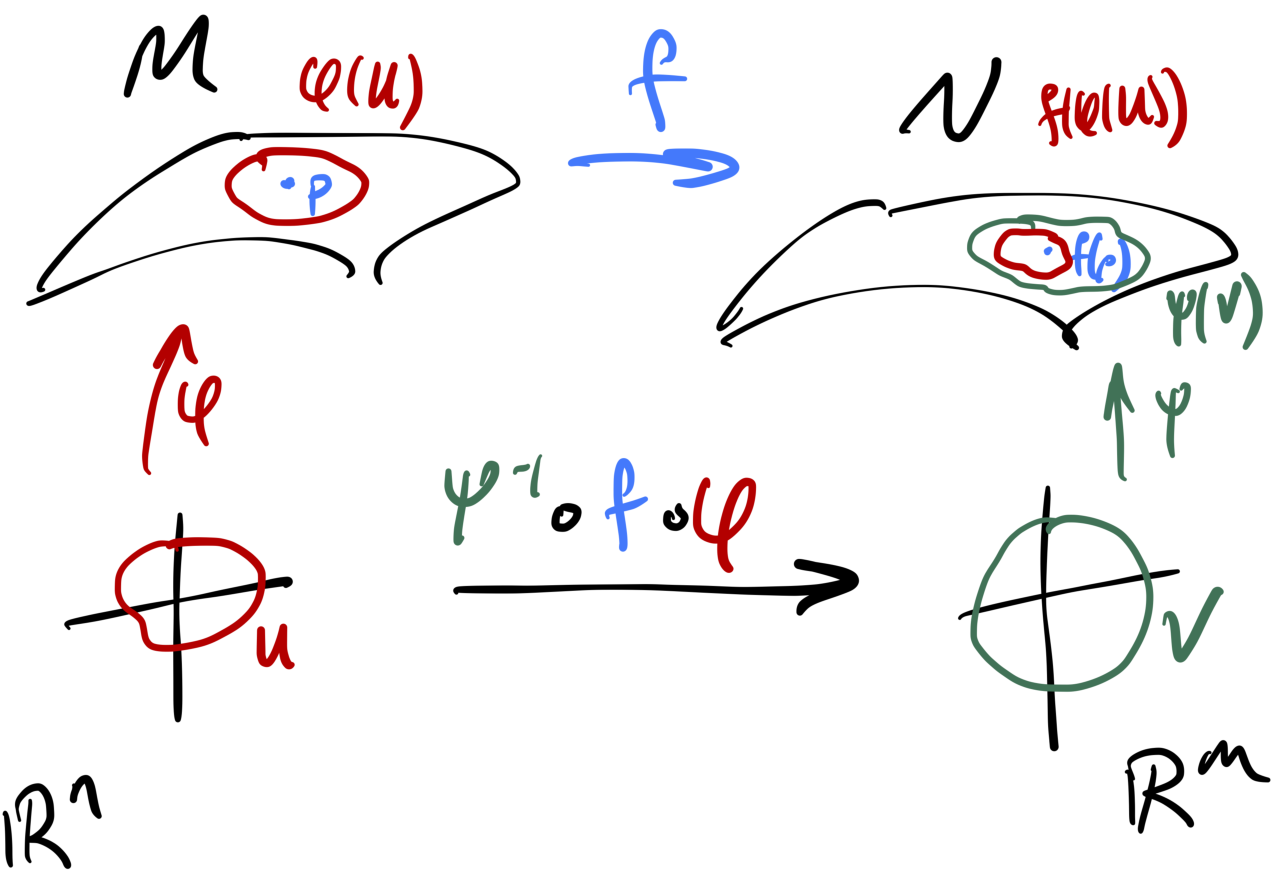
\includegraphics[height=2in]{differentiability}
	\caption{Locally converting a map between manifolds to a map between open sets in Euclidean spaces, where we know what differentiability means.}
	\label{fig:differentiable}
\end{figure}

% Add discussion of why \ref{it:manifold def overlap} implies that if there is \emph{some} coordinate chart in which $\psi^{-1} \circ f \circ \phi$ is smooth, then it will be smooth in \emph{every} coordinate chart.

\begin{example}
	Consider the antipodal map $\alpha \from S^n \to S^n$ given by $\alpha(\vec{y}) = -\vec{y}$. Then, so long as $\vec{y}$ is not the south pole, $\alpha(\vec{y}) = -\vec{y} \in \phi_N(\R^n)$ so we can take $\psi = \phi_N$ and $V = \R^n$. Moreover, $\vec{y} \in \phi_S(\R^n)$ so we can $\phi = \phi_S$ and $U = \R^n$, since $\alpha(\phi_S(\R^n)) = S^n \backslash\{N\} = \phi_N(\R^n)$. Then a straightforward calculation shows that
	\[
		(\phi_N^{-1} \circ \alpha \circ \phi_S)(\vec{x}) = -\vec{x},
	\]
	which is definitely differentiable everywhere (as a map $\R^n \to \R^n$). 
	
	Of course, if $\vec{y} = S$, we can swap the roles of $\phi_N$ and $\phi_S$ in the above, and we conclude that $\alpha$ is differentiable everywhere on $S^n$.
\end{example}

While we've given the definition of a manifold and of a differentiable map in this section, we generally try to use them directly as little as possible. They are hard to handle and fairly unintuitive, so we will quickly be looking for alternative ways of characterizing manifolds and differentiable maps.


% % !TEX root = ../dg.tex

\section{Tangent Vectors}

Notice that there's nothing in \cref{def:manifold} that says that a manifold has to live inside some bigger Euclidean space. This is in contrast to a typical undergraduate differential geometry course (like MATH 474 here at CSU), which is typically focused on surfaces in $\R^3$. 

Of course, many manifolds (like spheres) do naturally live in some Euclidean space, and it turns out that the Whitney embedding theorem~\cite{whitneySelfintersectionsSmoothnmanifold1944,whitneySingularitiesSmoothnmanifold1944} guarantees that all manifolds \emph{can} be embedded in some Euclidean space, but this embedding is not necessarily going to be pleasant to work with. If you've encountered them before, it is often much easier to work with projective spaces and Grassmannians \emph{without} embedding them anywhere in particular.

Since our manifolds don't necessarily live inside a Euclidean space, we have to be a bit careful about what a tangent vector at a point is supposed to be. In particular, a tangent vector at a point lives in a different universe than the point itself: the point is a point in the manifold, but the tangent vector does \emph{not} live on the manifold. This is clear even on a sphere in Euclidean space: the tangent vector to a point on the sphere does not live on the sphere! However, in Euclidean space we can kind of cheat and think of both the point and the tangent vector as both living inside the ambient Euclidean space. In general, we can't get away with this.

Now even in Euclidean space you have to be a little careful with this mixing of point and tangent vector: the tangent vector can't be any \emph{arbitrary} vector in the ambient Euclidean space: it has to lie in the \emph{tangent space} at the point, which we usually visualize as some plane which is tangent to the sphere at the point. But if we're not in Euclidean space, things are even worse: if there's supposed to be some subspace which is ``tangent at a point,'' where does it even live? Surely not in the manifold itself, but we're not thinking of the manifold as sitting inside some bigger space, so there's no ``outside'' where it can be.

This is a surprisingly nontrivial issue, requiring us to construct some abstract vector space which doesn't really live anywhere in particular. The construction is fairly non-obvious, and feels like a sneaky trick the first few times you encounter it. This is one of those situations where it seems like you're turning a concept inside-out; at least for me, the first time I encountered the following way of thinking, it made me feel uncomfortable in a similar way to when I first encountered the natural embedding of a vector space into its double dual. I will say that at some point my brain switched from ``this is weird and awkward'' to ``this is obviously the right way to do it'' and I think most differential geometers have had similar experiences, so this is something you can eventually develop intuition for.

% Add something about how ``varying the input a little bit'' can really only mean moving along some curve through the point.

Given that preamble, what's the idea? We're going to work by analogy with a way of thinking about vectors in $\R^n$ that's slightly different from what you may be used to. In words, we'll identify a vector $\vec{v} \in \R^n$ with the operator on differentiable functions which gives the directional derivative (in the direction of $\vec{v}$) of a function. 

That's a little vague, so let's try to characterize a tangent vector $\vec{v}$ to a point $p \in \R^n$ in this way (here I'm using the notation $p$ rather than $\vec{p}$, because I'm just thinking of $p$ as a point in a manifold, not as an element of a vector space). Given $\vec{v}$, I claim we can find some smooth curve $\alpha\from (-\epsilon, \epsilon) \to \R^n$ with $\alpha(0) = p$ and $\alpha'(0) = \vec{v}$; see \cref{fig:tangent vector curve}. In coordinates, if
\[
	\alpha(t) = (x_1(t), \dots , x_n(t)) \quad \text{for } t \in (-\epsilon, \epsilon),
\]
where the coordinate functions $x_i\from (-\epsilon,\epsilon) \to \R$ are themselves smooth, then
\[
	\alpha'(0) = (x_1'(0), \dots , x_n'(0)) = \vec{v}.
\]

\begin{figure}[htbp]
	\centering
		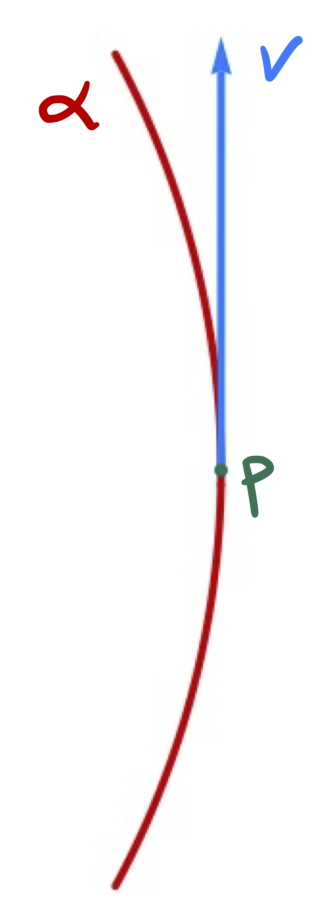
\includegraphics[height=2in]{tangent-vector-curve}
	\caption{A curve through $p$ with velocity $\vec{v}$ at $p$.}
	\label{fig:tangent vector curve}
\end{figure}

(In this specific case, we could take $\alpha(t) = p + t\vec{v}$, but it turns out not to matter which curve satisfying $\alpha(0) = p$ and $\alpha'(0) = \vec{v}$ we take.)

Now, say $f: U \to \R$ is differentiable, where $U \subseteq \R^n$ is some neighborhood of $p$. Then the directional derivative of $f$ at $p$ in the direction of $\vec{v}$ is 
\[
	\left. \frac{d(f \circ \alpha)}{dt} \right|_{t=0} = \sum_{i=1}^n \left.\frac{\partial f}{\partial x_i}\right|_p \left. \frac{d x_i}{dt} \right|_{t=0} = \left(\sum_{i=1}^n x_i'(0) \frac{\partial}{\partial x_i}]\right)f
\]
by the Chain Rule. 

On the right hand side above, we've written the directional derivative as an operator $L = \sum_{i=1}^n x_i'(0) \frac{\partial}{\partial x_i}$ acting on $f$. Moreover, this operator depends uniquely on $\vec{v}$ and is a \emph{linear derivation}, meaning that:
\begin{enumerate}
	\item \label{it:linearity of vector field} $L(f + \lambda g) = L(f) + \lambda L(g)$ for all $f$ and $g$ differentiable in a neighborhood of $p$ and all $\lambda \in \R$;
	\item $L(f g) = f(p) L(g) + g(p) L(f)$ (i.e., the Product Rule).
\end{enumerate}

If it's not clear to you, it's worth looking at the above and convincing yourself that the operator $L$ didn't really depend on the choice of $\alpha$: it really only depends on $p$ and $\vec{v}$ (you may need to go back to the justification from MATH 517 that the directional derivative is well-defined).

The upshot is that, given a point $p$ and a tangent vector $\vec{v}$ at $p$, we get a directional derivative operator $L$. And, conversely, if we know how to compute a directional derivative, we (at least implicitly) know the direction, so this is really a bijective correspondence.

The benefit of thinking in this way is that we can talk about differential operators like $L$ on any manifold; after all, manifolds locally look like $\R^n$ by definition. So, with that long preamble in mind, here's the definition of a tangent vector:

\begin{definition}\label{def:tangent vector}
	Let $M^n$ be a manifold. A smooth function $\alpha\from (-\epsilon, \epsilon) \to M$ is a (smooth) curve in $M$. Suppose $\alpha(0) = p \in M$ and let $\mathcal{D}_p$ be the set of function on $M$ that are differentiable in a neighborhood of $p$. The \emph{tangent vector} to a curve $\alpha$ at $t=0$ is a function $\alpha'(0)\from \mathcal{D}_p \to \R$ given by
	\[
		\alpha'(0)f := \left. \frac{d(f\circ \alpha)}{dt} \right|_{t=0} = (f\circ \alpha)'(0).
	\] 
	A \emph{tangent vector at $p$} is the tangent vector at $t=0$ of some curve $\alpha\from (-\epsilon, \epsilon) \to M$ with $\alpha(0) = p$.
	
	The set of all tangent vectors at $p$ is the \emph{tangent space} to $M$ at $p$, denoted $T_pM$.
\end{definition}

This is a nice coordinate-free way of defining things, but it's not very useful for computations. We usually \emph{do} want to work in coordinates for computations (and certainly for any computations that we want to do on the computer), so let's see what all this means in local coordinates.

Say that $(U,\phi)$ is a coordinate chart containing $p \in M$ so that $\phi(\vec{0}) = p$, that $\alpha \from (-\epsilon , \epsilon) \to M$ is smooth with $\alpha(0) = p$, and that $f$ is a differentiable function in a neighborhood of $p$. Then
\[
	(\phi^{-1} \circ \alpha)(t) = (x_1(t), \dots , x_n(t))
\]
for some smooth functions $x_1 , \dots , x_n\from (-\epsilon, \epsilon) \to \R$. Then
\[
	\alpha'(0) f = \left. \frac{d(f \circ \alpha)}{dt} \right|_{t = 0} = \left. \frac{d}{dt} (f \circ \phi(x_1(t),\dots , x_n(t))) \right|_{t=0} = \left.\sum_{i=1}^n x_i'(0) \frac{\partial f}{\partial x_i}\right|_{\vec{0}} = \left( \left.\sum_{i=1}^n x_i'(0) \frac{\partial }{\partial x_i}\right|_{\vec{0}}\right)f,
\]
where I'm using a very common abuse of notation in the second expression to think of $f$ as being a function on the coordinate chart $U$, and hence a function of coordinates $x_1, \dots , x_n$ (of course, it's really $f \circ \phi$ which is a function of $x_1, \dots , x_n$, as we see in the middle expression).

This all means that we can write the tangent vector $\alpha'(0) \in T_pM$ in local coordinates as
\[
	\alpha'(0) = \sum_{i=1}^n x_i'(0) \left(\frac{\partial}{\partial x_i}\right)_{\vec{0}}.
\]
Since the $x_i'(0)$ are just scalars, what we're doing here is writing $\alpha'(0)$ in terms of the \emph{local coordinate basis} $\left\{\left(\frac{\partial}{\partial x_1}\right)_{\vec{0}}, \dots , \left(\frac{\partial}{\partial x_n}\right)_{\vec{0}}\right\}$ for $T_pM$ associated to the chart $(U,\phi)$.

\begin{remark}
	In practice, we will almost always drop the subscript $\vec{0}$ and just write the basis as $\left\{\frac{\partial}{\partial x_1}, \dots , \frac{\partial}{\partial x_n}\right\}$ and generic tangent vectors as $\sum_{i=1}^n a_i \frac{\partial}{\partial x_i}$.
\end{remark}

\begin{exercise}
	Suppose a point $p \in M$ lies in two different coordinate charts. How are the two different local coordinate bases related?
\end{exercise}

% Add example with tangent vectors on the sphere using stereographic projection.

It's extremely important to keep in mind that, if $p$ and $q$ are distinct points on $M$, then the tangent spaces $T_pM$ and $T_qM$ are \emph{completely different vector spaces} that in principle have nothing to do with each other (they're both vector spaces of the same dimension, and hence abstractly isomorphic, but that's essentially all we can know without more detailed information about the geometry of $M$).

Nonetheless, we often want to talk about all tangent spaces at once, so we smush them together:

\begin{definition}\label{def:tangent bundle}
	The \emph{tangent bundle} of a manifold $M$, denoted $TM$, is the (disjoint) union of tangent spaces
	\[
		TM := \bigsqcup_{p \in M} T_p M.
	\]
	Likewise, if $(T_pM)^\ast$ is the dual of $T_pM$, then the \emph{cotangent bundle} is the union of cotangent spaces
	\[
		T^\ast M := \bigsqcup_{p \in M} (T_pM)^\ast.
	\]
\end{definition}

Notice that there are natural projections $\pi: TM \to M$ and $\widetilde{\pi}: T^\ast M \to M$ which just record the base point; in other words, $\pi$ sends a tangent vector at a point to the point (formally, $TM$ and $T^\ast M$ are \emph{vector bundles}, and this projection is part of their definition).

\begin{theorem}\label{thm:tangent bundles are manifolds}
	If $M$ is an $n$-dimensional manifold, then $TM$ and $T^\ast M$ are $2n$-dimensional manifolds.
\end{theorem}

\begin{exercise}
	Prove \cref{thm:tangent bundles are manifolds}.
\end{exercise}

$T^\ast M$ is, in some sense, the most basic example of a \emph{symplectic manifold}. In physics and dynamical systems language, if $M$ is the \emph{configuration space}\footnote{Meaning it records the positions of particles; for example if we're doing dynamics of $n$ points on the circle, the configuration space is the $n$-torus $S^1 \times \dots \times S^1 = (S^1)^n$.} of a (classical) system, then $T^\ast M$ is \emph{phase space} or \emph{position-momentum space}: this is the natural setting of Hamiltonian mechanics.

\begin{example}
	$T \R^n \cong \R^n \times \R^n \cong \R^{2n}$.
\end{example}

\begin{example}
	$T S^1 \cong S^1 \times \R$, the infinite cylinder.
\end{example}

\begin{example}
	$TS^2$ is a \emph{non-trivial} bundle over $S^2$, meaning that it is \emph{not} homeomorphic to $S^2 \times \R^2$. In particular, one can show that $US^2$, which is the \emph{unit} tangent bundle (the subset of the tangent bundle consisting only of unit tangent vectors) is homeomorphic to $\SO(3) \cong \RP^3$, the real projective space, which is a circle bundle over $S^2$ different from the trivial circle bundle $S^2 \times S^1$. (For those that have taken graduate topology, $\pi_1(S^2 \times S^1) \cong \Z$, whereas $\pi_1(\RP^3) \cong \Z/2\Z$.)
\end{example}


	
	



\printbibliography

\end{document}
